\documentclass[10pt, a4paper, spanish]{article}
\usepackage[paper=a4paper, left=1.5cm, right=1.5cm, bottom=1.5cm, top=3.5cm]{geometry}
\usepackage[utf8]{inputenc}
\usepackage[spanish,es-nodecimaldot]{babel}
\usepackage{caratula}
\usepackage[pdfencoding=auto, colorlinks=true, linkcolor=blue]{hyperref}
\usepackage[boxruled, longend]{algorithm2e}
\usepackage{wrapfig}
% \usepackage{tikz}
\usepackage[rightcaption]{sidecap}
% \usetikzlibrary{babel}
\usepackage{float}
\graphicspath{imagenes/}

% \tikzset{nodeList/.style={every node/.style={draw, circle}}}
% \tikzset{pathList/.style={every node/.style={midway, fill=white}}}


\newcommand{\ord}{\ensuremath{\operatorname{O}}}
\newcommand{\nat}{\ensuremath{\mathbb{N}}}

\begin{document}
% CARATULA
\materia{Métodos Numéricos}
\submateria{Segundo Cuatrimestre de 2017}
\fecha{\today}
\grupo{Fuerte a Pachi}
\titulo{Trabajo Práctico 2}

\integrante{Tarrío, Ignacio}{363/15}{itarrio@dc.uba.ar}
\integrante{Szperling, Sebastián Ariel}{763/15}{sszperling@dc.uba.ar}
\integrante{Mena, Manuel}{313/14}{manuelmena1993@gmail.com}
\integrante{Frachtenberg Goldsmit, Kevin}{247/14}{kevinfra94@gmail.com}

\maketitle

\newpage
\tableofcontents

\newpage
\section{Introducción}

Este trabajo práctico tiene como objetivo el desarrollo y estudio de una herramienta que permita reconocer dígitos manuscritos en imágenes. El algoritmo capaz de llevar esto a cabo es uno de clasificación supervisado que fue entrenado con un lote de caracteres conocido, de modo que le sea posible reconocer otras instancias de esos caracteres aprendidos que no se encuentren en la base de datos de entrenamiento.

En cuanto al reconocimiento de dígitos, estos serán entre el 0 y el 9, y estarán plasmados en imágenes en escalas de grises.

El resultado del algoritmo final fue medido con distintas métricas (HABLAR DE RECALL, PRECISION Y BLABLA).

\newpage
\section{Desarrollo}

\subsection{kNN}

El algorimo kNN (k Nearest Neighbours) se basa en el análisis de un conjunto de puntos del espacio para determinar a qué clase corresponde el nuevo objeto. En este caso cada imagen estara representada como un vector donde cada elemento es un píxel distinto de la misma. El conjunto de puntos elegido serán aquellas $k$ imágenes que más cerca se encuentren de la imágen a clasificar. Lo que se hace es clasificar a la nueva imágen como la clase que mayor representantes tenga en este conjunto de puntos cercanos.

Este algoritmo puede ser sumamente costoso en cuanto al tiempo de cómputo, y si la dimensión de los puntos a clasificar es muy grande, hacer uso del mismo podría resultar impracticable. Es por esto que se implemento un método cuyo objetivo es preprocesar las imágenes para reducir la cantidad de dimensiones de las muestras, permitiendo a kNN trabajar con muestras con una cantidad de variables menor. Este método es conocido como PCA (Principal components analysis).

\subsection{PCA}

El método de análisis de componentes principales se encarga de cambiar de base el conjunto de datos de entrada, reduciendo la dimensión de cada elemento tanto como se desee. Al reducir la dimensión de un punto es claro que se pierde determinada información sobre el mismo, pero la particularidad de este método es que, como su nombre lo indica, se queda con las componentes más importantes, dejando de lado las que menos información aporten. De este modo, la información que se descarta es la que menor relevancia tiene, por lo que se lo considera una buena manera de reducir el espacio de la entrada.

Es importante aclarar que el método no solamente reduce la dimensión de los datos, sino que cambia la base de los mismo. Por lo que es necesario tener esto en cuenta al momento de trabajar con los mismos. Si se utiliza este método para reducir la entrada de kNN, es necesario cambiar a la misma base la imagen a clasificar, de lo contrario estarían comparándose elementos que viven en distintos espacios.

\bigskip

Procedimiento para el cambio de base:

\begin{enumerate}
\item Siendo $X$ la matriz cuyas filas contienen las imágenes, se calcula $\mu = (x_1 + ... + x_n)/n$ el promedio de las imágenes, donde $x_i$ es la $i$-ésima imagen.
\item Se crea la matriz $X_\mu$ que contiene en la $i$-ésima fila al vector $(x_i - \mu)^t$
\item Se calcula la matriz de covarianza $M = X_\mu^tX_\mu$
\item Se calculan los autovectores de $M$ mediante el método de las potencias, con deflación. Cómo cada iteración en la que calculamos el autovector de la matriz en cuestión, este está asociado al autovalor de máximo módulo, los autovectores que habremos calculado se encontrarán ordenados por relevancia. De esta manera se calculan tan solo $\alpha$ autovectores, con $1 \geq \alpha \geq n$, siendo $\alpha$ la dimensión a la que se quiere reducir las imágenes.
\item Se contruye la matriz $V$ con los autovectores caluclados previamente, dispuestos como columnas. $V$ es la matriz de cambio de base.
\item Por último, se reduce la dimensión de $X$ cambiando su base. El resultado final es $V^tX^t$ que contiene la misma cantidad de imágenes pero expresadas en otra base, y en lugar de tener dimensión $n$, cada una tiene dimensión $\alpha$.
\end{enumerate}\tabularnewline

Puede que sea interesante notar que una vez hecho el cambio de base de las imágenes, éstas representan a las imágenes pero si se trata de graficarlas se obtendrá algo muy distinto a lo que era anteriormente y no podrá visualizarse nada en concreto. Solo volviendo a la base original sería posible, pero ya se habrá perdido mucha información por lo que probablemente sea difícil encontrarlo útil.



\newpage
\section{Resultados}

Uno de los objetivos de la experimentación de este trabajo práctico era encontrar los mejores parámetros para los métodos, es decir, los parámetros para los cuales los algoritmos proporcionaban mejores resultados. Para determinar la calidad de los resultados obtenidos (cuáles eran los mejores) se tuvo en cuenta distintas métricas, que ayudaron a determinar esto mismo:

\begin{itemize}
\item Accuracy
\item F1-Score
\end{itemize}

Los resultados obtenidos fueron analisados en términos de estas métricas aplicando validación cruzada \textit{K-fold} (sobre la cual se hablará a continuación) sobre la base de entrenamiento.

Los parámetros $k$ (cantidad de vecinos en \textit{kNN}) y $\alpha$ (dimensión a la cual se reduce cada imagen con \textit{PCA}) fueron variándose como se expondrá en las páginas siguientes.

\subsection{K-fold}

La validación cruzada \textit{K-fold} consiste en particionar la base de entrenamiento en $K$ partes del mismo tamaño. Luego se realiza $K$ iteraciones, cada una de ellas reteniendo uno de los conjuntos para validación y utilizando los restantes $K - 1s$ para entrenamiento. Este método puede ser aleatorio, es decir, tomar las particiones sin cuidado alguno. Hicimos uso del método de MATLAB cvpartition, la cual tiene como define las particiones aleatoriamente de la cross-validation para un $n$ y un $K$.

\subsection{Tiempo de ejecución}

Medimos 2 cosas en términos de los tiempos de ejecución: el tiempo que toma realizar PCA sobre el set de entrenamiento, y el tiempo en aplicar kNN sobre uno de los elementos (incluyendo el cambio de base en el caso de haber realizado PCA).

Para estas mediciones tomamos los sets de entrenamiento y prueba provistos por la cátedra, correspondientes a la competencia de Kaggle. También usamos para estas pruebas $k = 10$ (para kNN) y $alpha = 100$ (para PCA). 

Los resultados fueron que, para el caso sin PCA, cada elemento de prueba tarda en promedio 500 ms en ser procesado. Consideramos que esto es relativamente lento, ya que al tratarse de 28,000 elementos, esto suma en total 3.89 horas, lo que resulta bastante prohibitivo y fue problemático a la hora de hacer experimentaciones.

En contraste, en el caso con PCA, cada elemento era procesado en aproximadamente 95ms, una mejora sustancial sobre todo considerando que esto incluye el cambio de base. Al aplicar sobre el set de prueba completo, esto demora alrededor de 45 minutos, una fracción del tiempo mencionado anteriormente.

Por último, cabe destacar que PCA en sí es un proceso costoso. Sin embargo, como nos esperábamos, el costo de PCA está compensado por las dimensiones de los sets utilizados, y aplicarlo sobre nuestro conjunto de entrenamiento demora en promedio 26 minutos, por lo que sumado a kNN, sigue representando apenas más del 25\% del tiempo de ejecución sin PCA.

Sin embargo, debe recordarse que el costo de PCA es elevado. Esto, junto con la precisión obtenida, debe tenerse en cuenta para sets de datos más pequeños, ya que podría no justificarse.

\subsection{K de Knn}

Para analizar el comportamiento al cambiar el K de Knn fijamos alfa de PCA en 2 valores 15 y 30. Corrimos experimentos para distintos estos K: 1, 2, 3, 4, 5, 7, 8, 8, 10, 15, 20, 30.

Nuestra hipótesis previo a correr los experimentos fue que para $k$s chicos, la posibilidad de que nuestro vecino más cercano sea un outlier representando otro dígito son más altas y para los $k$s grandes, pensamos que los dígitos que se encuentran en las fronteras, osea que se parecen a otros dígitos, se verían perjudicadas ya que por como funciona knn, pordía ocurrir que el más cercano sea, por ejemplo, 5 pero todos los siguientes sean 2. Por lo tanto, supusimos que los $k$s intermedios serían los que mejor funcionarían.

Habiendo corrido los experimentos, el gráfico de accuracy generado fue el siguiente:

\begin{figure}[H]
    \begin{center}
      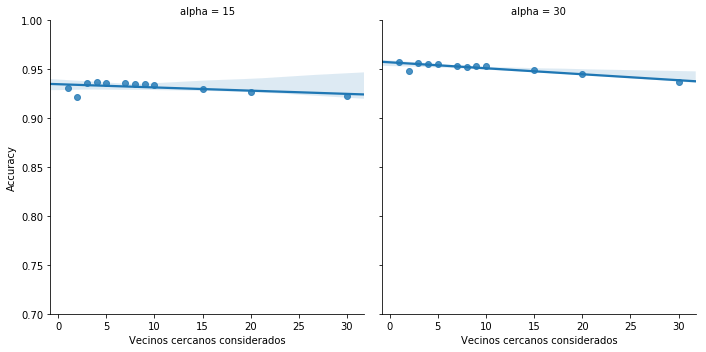
\includegraphics[width=0.8\columnwidth]{imagenes/Accuracy_15_30.png}
      \caption{Accuracy por k de kNN con alfa de PCA fijo}
    \end{center}
\end{figure}

Lo que se observó en este gráfico fue que el algoritmo es estable para los distintos $k$s y que las diferencias fueron poco significativas, pero pudimos contrastar con la hipótesis que lo que propusimos estaba en lo correcto.

El siguiente gráfico es una comparación del F1 score sobre los mismos resultados anteriores.

\begin{figure}[H]
    \begin{center}
      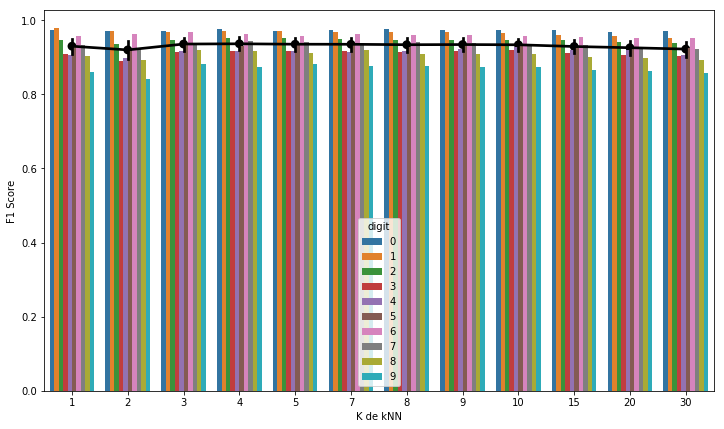
\includegraphics[width=0.8\columnwidth]{imagenes/F1_alpha_15.png}
      \caption{F1 score por k de kNN con alfa de PCA fijo en 15}
    \end{center}
\end{figure}

\begin{figure}[H]
    \begin{center}
      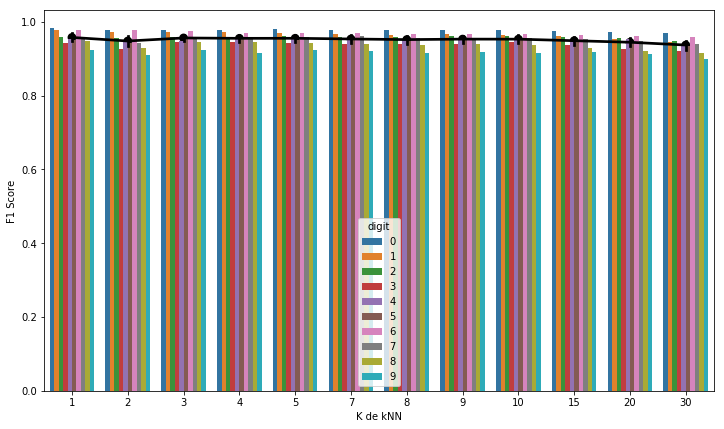
\includegraphics[width=0.8\columnwidth]{imagenes/F1_alpha_30.png}
      \caption{F1 score por k de kNN con alfa de PCA fijo en 30}
    \end{center}
\end{figure}

Este gráfico nos mostró también que el algoritmo es estable para cada dígito y que para alfa 30 de PCA las diferencias entre los dígitos es menor. En la siguiente sección entraremos en detalle sobre la comparación que realizamos sobre el alfa de PCA.

\subsection{Alfa de PCA}

El otro parámetro que tratamos de optimizar fue el alfa de PCA, de una forma similar al K, fijamos este y fuimos cambiando el alfa, por suerte ya teníamos resultados sobre el K, así que decidimos fijarlo en 5. Los alfas con los que experimentamos fueron: 5, 10, 15, 20, 25, 30, 40, 50, 60, 80, 100, 150

% chamuyar con los graficos obtenidos
% hablar sobre proporcion de duracion de experimento entre 30 y 50

\subsection{Data augmentation}

Antes de entrenar el algoritmo con todo el dataset quisimos ver cómo el modelo de transformaciones escalaba, para eso corrimos sobre un subconjunto del set de datos, a los mismos 10k digitos les aplicamos la transformación para obtener así un dataset de 20k. Como ya teníamos el K y el alfa analizados usamos 5 y 30 respectivamente. Los resultados del experimento fueron una accuracy de 0.9602 para las rotaciones y de 0.9715 para las deformaciones elásticas. Pudimos apreciar una gran mejora con las deformaciones elásticas, esto se puede deber a que las rotaciones hay casos en los que no queda tan real el dígito generado.

\newpage
\section{Apéndice}

\subsection{Apéndice I: detalles de implementación}

Para poder soportar la posible necesidad de matrices más eficientes en memoria, creamos una clase Matrix con múltiples implementaciones. La misma tiene métodos para cada operación que consideramos necesaria, y algunas otras utilidades que utilizamos en el Trabajo Práctico 1. Por otro lado, implementamos una matriz completa (con vectores de la biblioteca estándar de C++), una matriz dispersa (usando mapas), y otras versiones más específicas.

Para evitar complicaciones con el manejo de punteros y el polimorfismo, utilizamos \texttt{std::shared\_ptr} de C++11, que se encarga de borrar las matrices que no necesitamos por nosotros.

Sin embargo, luego nos dimos cuenta que los casos de uso de este TP no requieren varias versiones especificas como si las requería tal vez el TP anterior. La implementación sigue incluída, pero solo se usa la versión completa de la matriz (denominada \texttt{FullMatrix}).

Otro elemento que dejamos en la implementación pero no se utiliza fueron unos pseudo-iteradores para las imágenes que recorren archivos en lugar de vectores en memoria. El mismo no se usa porque es muy poco eficiente (ya que lee múltiples veces un archivo en disco), y luego de medir el consumo de memoria lo consideramos innecesario.

Por otro lado, decidimos abstraer el entrenamiento y el reconocimiento de las imágenes en una clase común, a modo de intercambiar implemetaciones rápidamente y por parámetros. Hoy en día nuestro TP solo cuenta con 2 implementaciones: kNN y kNN + PCA, pero podrían argegarse otras variaciones a futuro.

\subsection{Apéndice II: código complementario en MATLAB}

Además del código con el reconocimiento de dígitos implementado en C++, incluímos en la entrega algunos scripts de MATLAB que nos resultaron útiles durante la experimentación. Los mismos incluyen comentarios explicando su funcionalidad, pero todos están relacionados a los datos con los que expermientamos (con algunos métodos para probar incrementando el set de entrenamiento) y los resultados de dichos experimentos (validación cruzada, F1 score, etc).

\subsection{Apéndice III: Gráficos e imágenes}

\begin{figure}[H]
    \begin{center}
      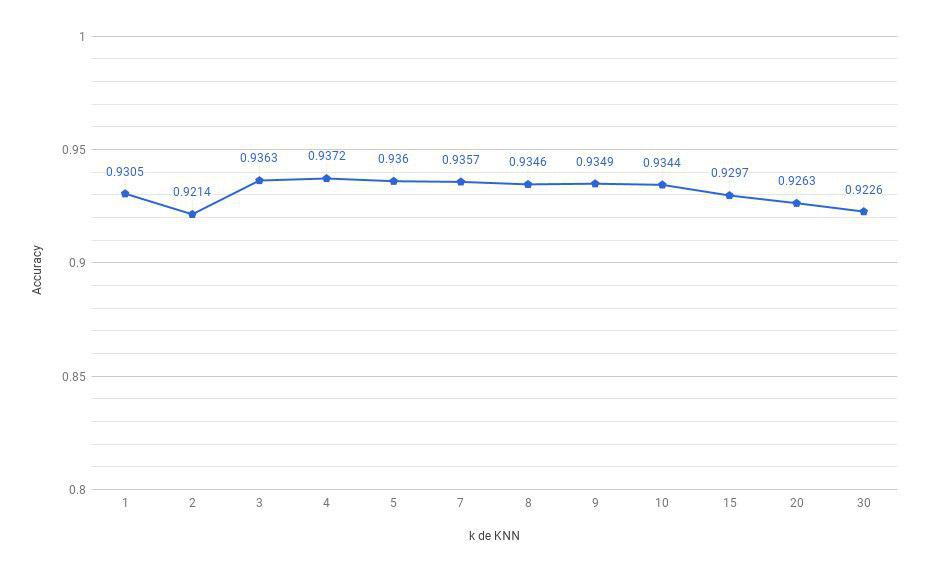
\includegraphics[width=0.8\columnwidth]{imagenes/knn-accuracy.jpg}
      \caption{Accuracy por k de kNN con alfa de PCA fijo en 15}
    \end{center}
\end{figure}

\begin{figure}[H]
    \begin{center}
      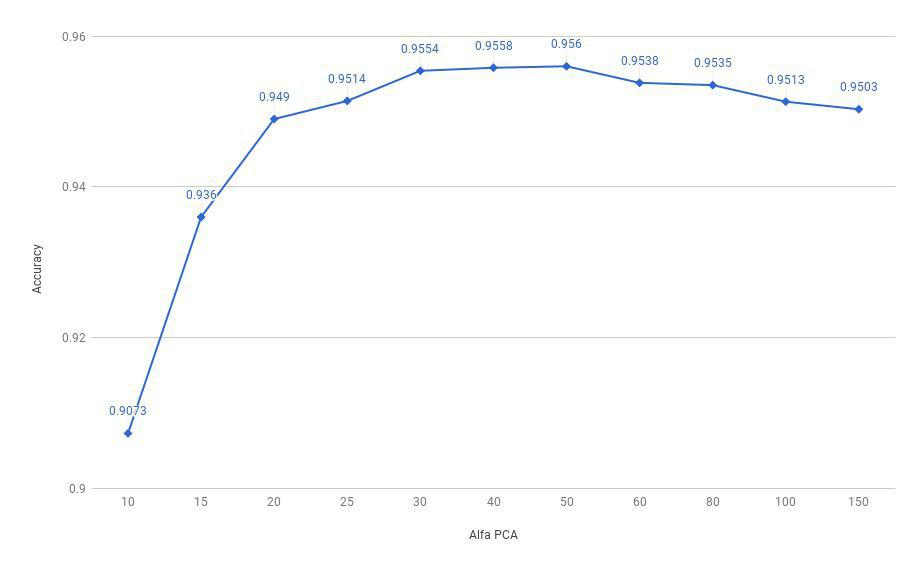
\includegraphics[width=0.8\columnwidth]{imagenes/pca-accuracy.jpg}
      \caption{Accuracy por alfa de PCA con k de KNN fijo en 5}
    \end{center}
\end{figure}

\begin{figure}[H]
    \begin{center}
      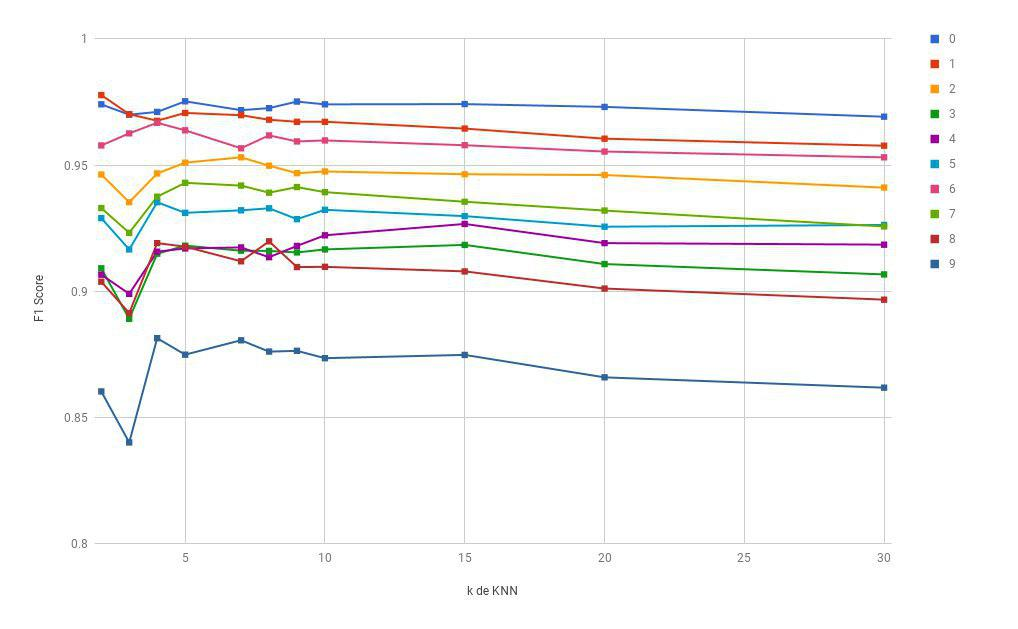
\includegraphics[width=0.8\columnwidth]{imagenes/knn-f1.jpg}
      \caption{F1 Score por k de kNN con alfa de PCA fijo en 15}
    \end{center}
\end{figure}

\begin{figure}[H]
    \begin{center}
      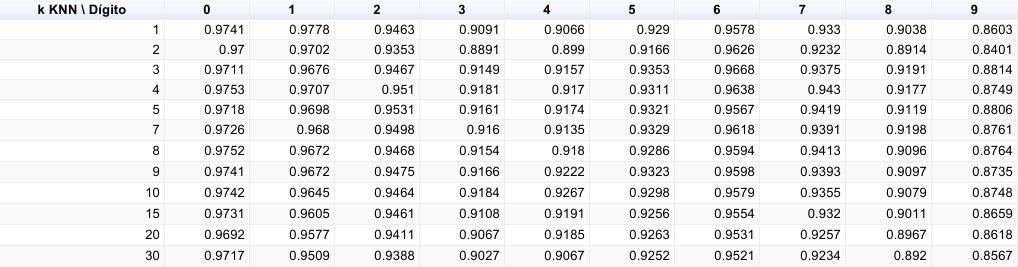
\includegraphics[width=0.8\columnwidth]{imagenes/knn-f1-table.jpg}
      \caption{F1 Score por k de kNN con alfa de PCA fijo en 15}
    \end{center}
\end{figure}

\begin{figure}[H]
    \begin{center}
      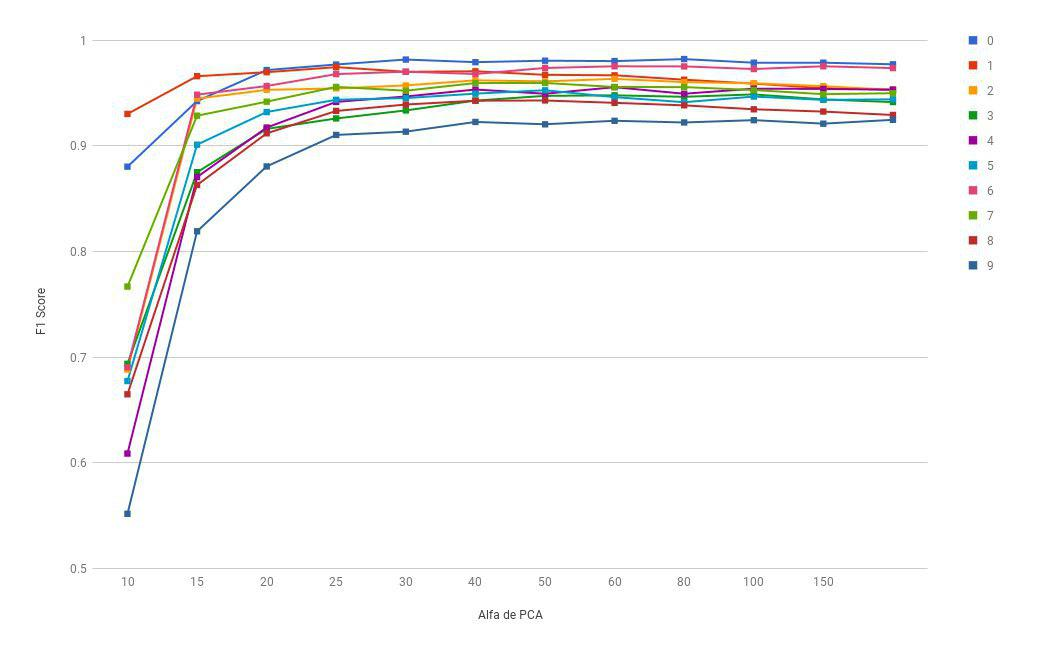
\includegraphics[width=0.8\columnwidth]{imagenes/pca-f1.jpg}
      \caption{F1 Score por alfa de PCA con k de KNN fijo en 5}
    \end{center}
\end{figure}

\begin{figure}[H]
    \begin{center}
      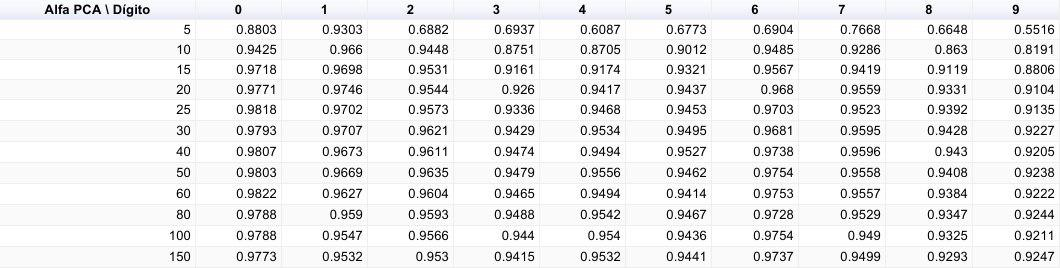
\includegraphics[width=0.8\columnwidth]{imagenes/pca-f1-table.jpg}
      \caption{F1 Score por alfa de PCA con k de KNN fijo en 5}
    \end{center}
\end{figure}

\begin{figure}[H]
    \begin{center}
      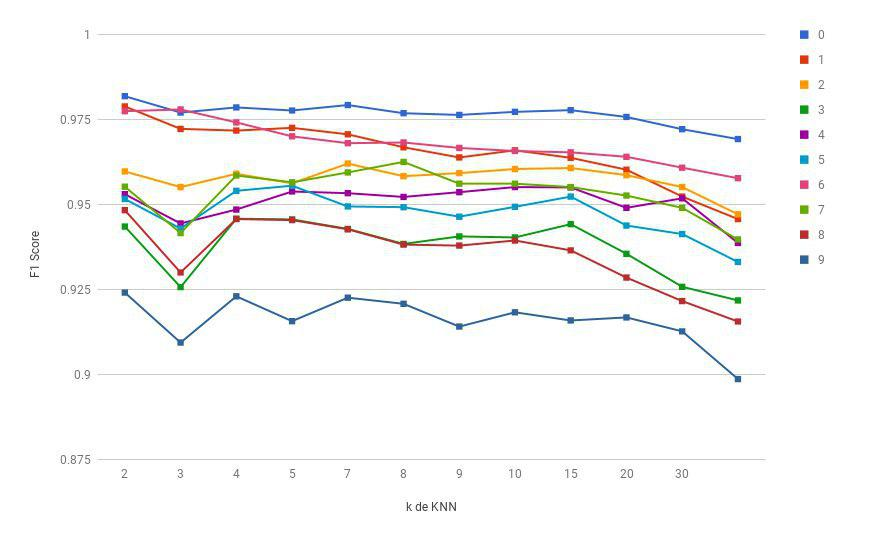
\includegraphics[width=0.8\columnwidth]{imagenes/knn-f1-pca30.jpg}
      \caption{F1 Score por k de KNN con alfa de PCA fijo en 30}
    \end{center}
\end{figure}

\begin{figure}[H]
    \begin{center}
      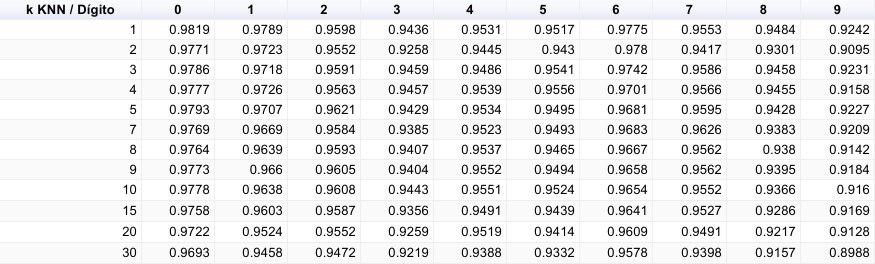
\includegraphics[width=0.8\columnwidth]{imagenes/knn-f1-table-pca30.jpg}
      \caption{F1 Score por k de KNN con alfa de PCA fijo en 30}
    \end{center}
\end{figure}

\begin{figure}[H]
    \begin{center}
      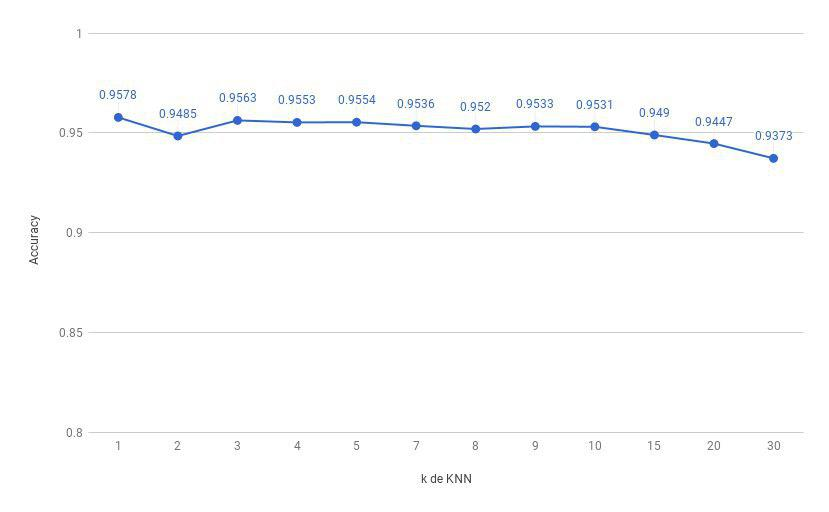
\includegraphics[width=0.8\columnwidth]{imagenes/knn-accuracy-pca30.jpg}
      \caption{Accuracy k de KNN con alfa de PCA fijo en 30}
    \end{center}
\end{figure}

% compilar 2 veces para actualizar las referencias


\end{document}